%*******************************************************************************
%*********************************** First Chapter *****************************
%*******************************************************************************

\chapter{Introduction}  %Title of the First Chapter 

\graphicspath{{Chapter1/Figures/} {Chapter1/Figures}}
\begin{quote}
\textsl{One should never try to prove anything that is not almost obvious - Alexander Grothendieck}
\end{quote}


\section{Introduction}

We live in a world where information is being bombarded on our cognitive faculties from all sides, at all times. The internet is a continuous stream of information and each source is fighting with the other to get a piece of our attention budget. 
With the advent of machine learning and big-data sources, building systems that predict actions as a response to perceptual triggers is the bread and butter of many companies. The use cases may range from understanding which advertise made a visitor do an unscheduled purchases on amazon, or which string of music tracks recommendations maximized a users time on a particular music platform. But in the end it all boils down to understanding what triggers result in human action or lack there of\cite{song2012survey}. Nonetheless the systems that surrounds a human interacting with the internet, are all figuring out the best triggers which are perceived by the human as worthy of attention. 
The term ``Attention Economy''\cite{davenport2001attention} was actually coined for this very reason. In the words of Matthew Crawford ``\textit{Attention is a resource, a person has only so much of it.}''\cite{MatthewCrawford}. We live in the age of distraction, and more often than not, our perceptions are guiding our actions, than our cognitive processes. Several studies have shown that engagement is almost always a game of stimulating our most basic urges, such as dopamine hits, presence of faces or simply arousal of emotions to increase the working memory.\cite{bakhshi2014faces,joglekar2017like}\cite{schupp2006emotion}\cite{soat2015social}. 


An interesting side effect of dwindling attention budgets is the emergence of more formal topical spaces on the internet. The ever pervasive nature of the internet allow these formal spaces to function almost like physical communities, with moderated and effective peer to peer exchange of thoughts, ideas and empathy\cite{kummervold2002social,squire2015should,hwang2010social}.
In such an environment, as computer scientists, it is worth asking the question: \textbf{Can we develop pipelines that can look at the structures in the data to quantify how humans perceive their sphere of interaction? Can we use that perception to design impactful interventions towards well being of the users, on and off the internet?}. 
This question can be decoupled into two fundamental problems:
\begin{enumerate}
\item How do human perceptions manifest in data? 
\item How do we quantify these perceptions?
\end{enumerate}
These two questions are going to be the guiding principles of my dissertation. 

But first of all, we need to clarify the relation between perception, affects and data. To do so we should try and understand each of these terms separately in the context of the field of application.

\section{Perception and Affect}
Across my work , I would try to build frameworks to capture human perceptions in the realm of human to human interactions and subjective intangible qualities like the sense of beauty or the sense of comfort. The utility of such an attempt, can only be justified if there is a real link between how humans function at the most fundamental cognitive level and how they perceive the intangible, including the aesthetic. There has been an ongoing effort to unravel this link, through psychological, neuro-evolutional and philosophical arguments. I will try to gain inspiration from them, but a detailed critique is beyond the scope of my dissertation and expertise\\
\textsl{\textbf{Affect (APA definition):} any experience of feeling or emotion, ranging from suffering to elation, from the simplest to the most complex sensations of feeling, and from the most normal to the most pathological emotional reactions.}\\
\textsl{\textbf{Perception (APA definition):} the process or result of becoming aware of objects, relationships, and events by means of the senses, which includes such activities as recognizing, observing, and discriminating. These activities enable organisms to organize and interpret the stimuli received into meaningful knowledge and to act in a coordinated manner.}\\

Emotions or `affects' and perceptions have long been discussed in the psychology, neuroscience and philosophical literature. Emanuel Kant in his prolific work, first discussed the utility and the philosophical reasoning behind presence of affects or emotions\cite{kant1987critique}. In his opinion, emotions are pre-cognitive involuntary states, termed as "mere perceptions of unspecified bodily states"\cite{borges2004can}. But that does not mean they don't influence our deepest level of well-being and influence our decision making processes.
The link between affect and perception has also been explored in several other cases. An argument to link perception of affect producing aesthetics was made by Perlovsky\cite{perlovsky2014aesthetic}, where they propose that the phenomenon of affects arousing from aesthetics, comes from a fundamental human need to enrich the knowledge about real world. An unexpected thing, stimuli or structure in physical space creates a dissonance between our expected model of the world and the perceived reality at some level and we perceive it as aesthetically pleasing. Another recent study by Zadra et.al\cite{zadra2011emotion} evaluated the relation between visual perception and emotions. They demonstrate that the conventional assumption of the disentangled functioning of perception and affects is not necessarily true. Humans are quite susceptible to perceiving different realities based on different aroused affects. 

The discussion on the formal definition and process of affects will continue, but there seems to be a consensus, at-least among the computer science and information science community that affects do influence our decisions and we perceive information through a filter of affects. Affective triggers can be generated when information is formatted or packaged in a certain way. In such a setup, it is worth testing if certain affect driven interactions on the web leave a trail of patterns in the data of these interactions. Furthermore it is work asking if these patterns might in some way be used to improve our online and physical environments.

\section{Intervention and the DIKW model}

\begin{figure*}[t!]
    \centering
    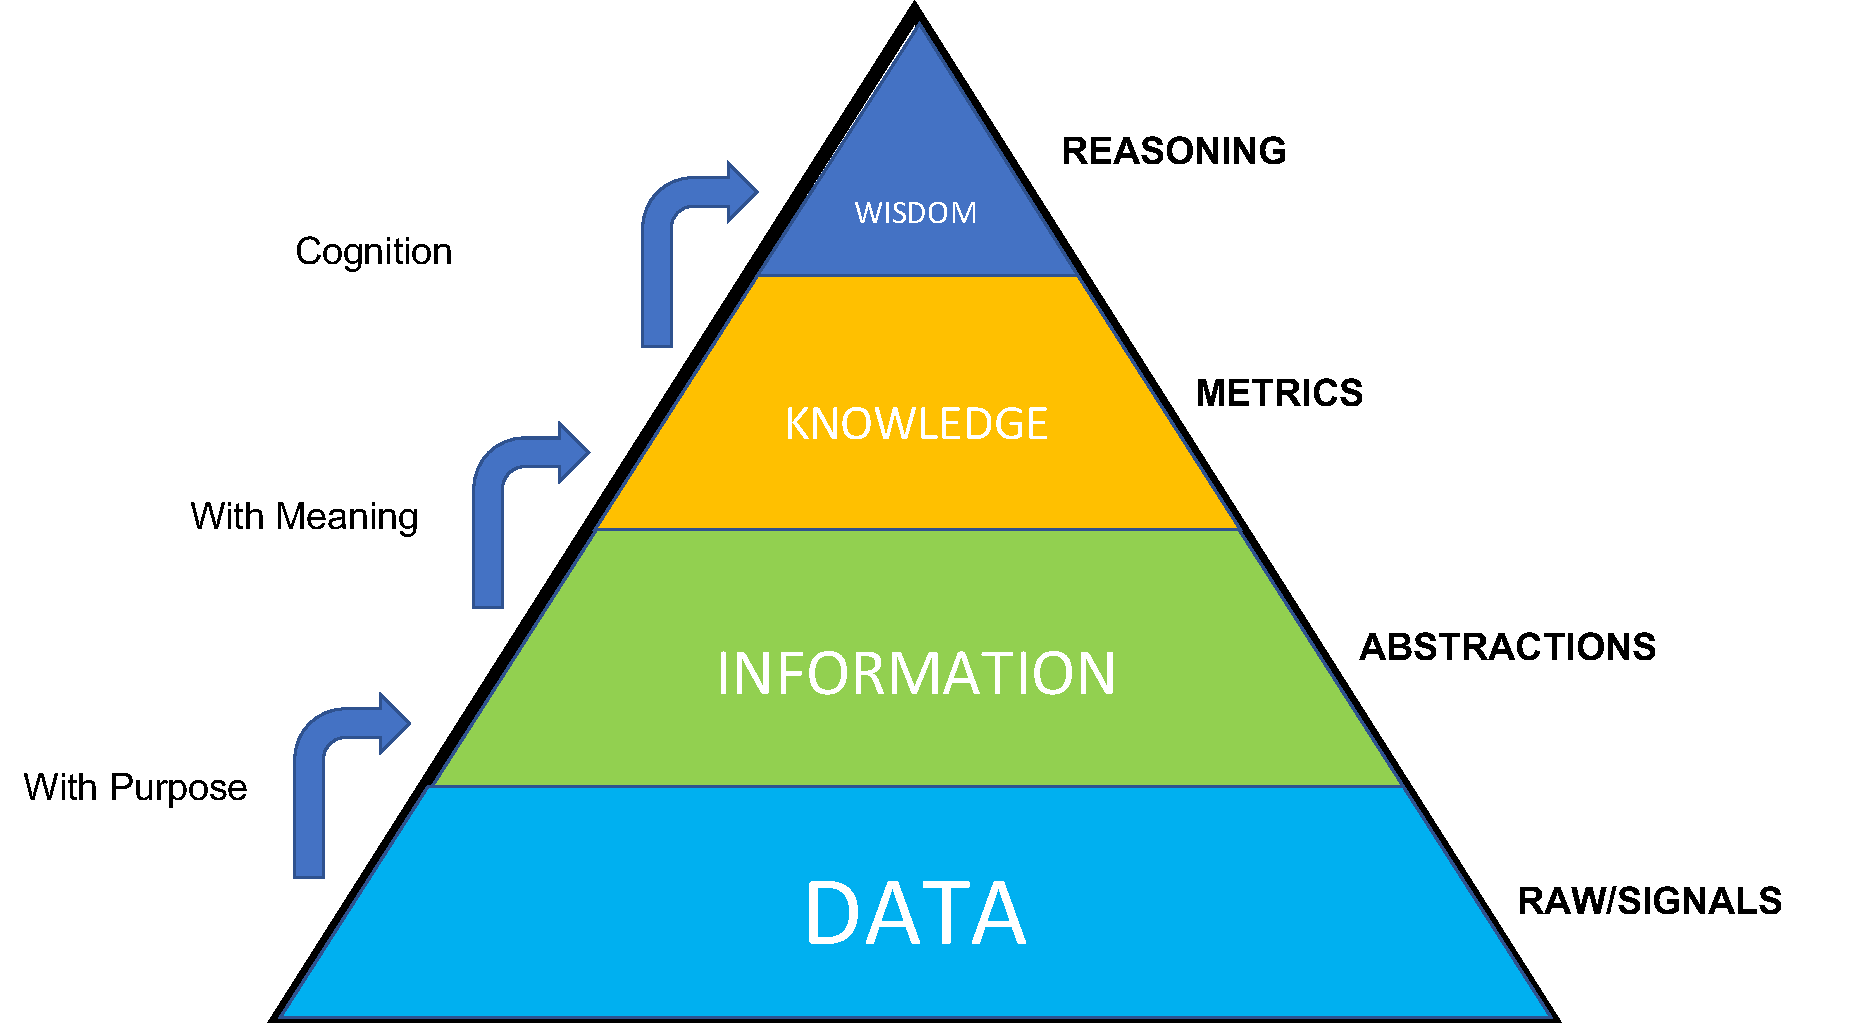
\includegraphics[width=\columnwidth]{DIKW.pdf}
    \caption{The DIKW pyramid}
    \label{fig:dikw}
\end{figure*}


The reflection to find the answers the questions enumerated before, ties us back to one of the fundamental frameworks about operations on data, that is the \textbf{Data , Information, Knowledge and Wisdom} model\cite{rowley2007wisdom}.In this dissertation I posit and demonstrate through case studies, that for any reasoning about perceptions and affects, you need to develop frameworks that extract knowledge from data in a format that is aligned with the ontological framework of the application. In the context of this dissertation, ontology implies a set of concepts, definitions and relations between these entities defined around a common set of axioms. Debating the nature of this ontology is not the purpose of this dissertation, but I show that `a' solution can be reached, if systems are designed to interpret metrics extracted from the data by anchoring around an ontological framework. But to reach this step, the data needs to pass through the 4 layers of the DIKW pyramid model.

In this model, the most base layer consists of the pure form raw \textbf{data or signals} that come from a source. If we are measuring perceptions of humans, this source needs to be tied back to humans in some way. The data needs to be generated as a result of some human-human interaction or as a result of deliberate human input as a form of response to their perception of some event. 

The \textbf{information} layer is the result of the fact that any process done on the data is with a sense of purpose or an end goal. For example, if the goal is to understand how humans exchange messages at times of distress, you would most certainly need to express the raw information about sender and recipient of messages into some form of a networked abstraction. The abstraction preserves the organization of data, but at the same time allows information to be operated on. As a result, almost always the output of this process is some form of a data abstraction. You need to attach some meaning to the patterns in the information to extract knowledge about the fundamental processes that you want to measure.

\textbf{Knowledge}. Defining knowledge has been an ongoing effort in the field of philosophy. But in the context of information science, knowledge involves collation of diverse sources of information and  mix of contextual information, values and metrics to deliver a coherent understanding of the real world. For example, if you need to know the most popular user among a social network of users exchanging messages; you would look for the most central user in the network(abstraction) along with several other temporal and structural metrics to arrive at a few candidates. In this particular case, these metrics, along with the context of the social network's design, dawns the meaning of popularity. 

The final layer needs a cognitive process and an ontological framework, to extract actionable insights, which we can call \textbf{wisdom}. By classical definition of ontology, it defines properties of and relations between objects or concepts. For this very reason, these ontological frameworks need to be originating from the fields of intervention.  In our example, lets assume we need to get some insights about the dynamics of popular users. Particularly in the context of optimizing advertising delivery. For example we need to understand how a particular piece of advertising, might percolate through the network if certain popular users advertise it. However to arrive at these insights we need to be grounded in the ontological frameworks of epidemiology, network physics and depending on the application, advertising or meme theory. Then using the abstractions of social networks, the metrics derived from them, and the ontological basis of all the aforementioned field, we might design a pipeline that could deliver us these insights to reasonable accuracy. 

Figure \ref{fig:dikw} shows an illustration of the adopted version of Rowley's DIKM model, which I would refer back as a repeating motif for my dissertation.

\subsection{Data}
To develop frameworks around quantification of human perceptions, such that we can do impactful interventions from this approach, we first need to make sure we formalize how we acquire, clean and condition our data. The most base level of this pyramid is the data that the frameworks would work with in order to progress on these lines. I work with diverse forms of data such as textual data , video data and image data to understand how these might exhibit signatures of human perceptive processes. 

\subsubsection{Textual Data}
The first case study of this dissertation focusses on is online support communities. It has been shown through several studies in medical informatics, that these communities play a very important role in providing support and respite in times of distress. The communities are especially helpful when it comes to people suffering from long term illnesses or mental health issues. 
To understand how users on these communities perceive social support, I work with data acquired from online health forums, where users share, give support and ask for support. I look at communities that deal with long term conditions like Lung illnesses, and communities where mental health patients seek support. 

\subsubsection{Image data}
The other facet of my work looks for quantification of how we perceive physical spaces. I work with google street view data, and with the aim to understand, through crowd sourced methods, how people perceive the sense of beauty in urban areas. Then using the ontological basis of urban design and architecture, can be design advanced machine learning driven frameworks to improve the real world spaces based on these quantified perceptions. =

\subsection{Abstractions}
As mentioned before, the act of aggregating information from data, almost always involves building organized abstractions. In case of the study with textual data, I incorporate user information into the textual data to build organized networked structures, which can then be evaluated using graph theoretic methods. To understand textual patters, I use the language embedding models which would be discussed in the chapters to come. To understand the social patterns among the conversations, I import concepts from social sciences about social ties.  
While working with image data, I use several segmentation techniques to group semantically similar pixels together. I also use several state of the art object and scene detection to extract semantic information from an image. I also use deep convolutional networks and generative models, to abstract out a representation of beauty. A more detailed discussion of these abstractions would be done in the later chapters.  

\subsection{Knowledge}
For extracting knowledge, we need to first associate meanings to certain computable metrics that we obtain from the abstractions. As discussed in the previous example, it could be as simple as associating the property of ``popularity'' to the metric of centrality. In my case, I develop several of these metrics for the two studies, some based on intuitions which I validate, and some based on extensive literature survey. To give an example, I develop the concept of anchored triads, which combines local interaction motifs with the role of a user in a supportive conversation, to understand how these conversations evolve. 

\subsection{Wisdom}
Finally the wisdom in my case, is simply the philosophical, quantitative and qualitative discussion about what perception did we actually capture from these operations. To answer the questions posed by this layer, we need to hold on to \textbf{an ontological framework} which grounds the metrics in the field of human interaction and planned intervention. This ontological framework that deems meaning to the structure in data, needs to be achieved through cross disciplinary literature review. In case of social support, what metrics combined with the understanding of human behavioural ontology, give rise to signatures of social support? Could those be found in sociological literature that distils social ties as interaction motifs? Or can that be found in pure statistical understanding of networks and formation of edges?  In the end, can we provide valuable interventions in the scenarios where humans are asking for help online. My dissertation navigates similar questions to arrive at 'an approach' to quantify and intervene using signatures of human perceptions from data.

\section{Research avenues}
The global hypothesis of my dissertation as described before comprises of asking the two aforementioned questions: \textbf{How do human perceptions manifest in data?} and \textbf{How do we quantify these perceptions?}. But these questions are quite open ended, and answering them in a generalized manner seems impractical. For this reason, I need to first contextualize my work in the realm  of practical applications. 
To rationalize the pursuit of these questions, I choose application driven case studies, which allow me the luxury to do a data driven exploration with a final goal of designing intervenable frameworks.
Across my investigations, I follow the DIKW framework layer by layer, by distilling actionable wisdom from data. Through the two case studies , my work touches a diverse set of data science tools  which range from complex networks formulations to generative adversarial models of human perception.

\subsection{Supportive Interactions on the web}
Humans are social animals in every aspect. The presence of social support systems in ones lives have shown to have huge quantifiable benefits. From speeding up recovery in cases of post-partum depression or in the cases of cancer survivors\cite{collins1993social,dunkel1984social,baron1990social} , to signs of positive turn around among patients suffering from alcoholism and depression \cite{peirce2000longitudinal,brown1986social}, social support is a key predictor of positive prognosis for patients under distress. With the advent of internet, a lot of communities have sprung up, which provide a rich platform for patients to interact, exchange support as well as provide a perceived sense of community. These communities do not have any special provisions for the users, but have an emergent behaviour of support and help by the very reason of homogenous membership. In other words, everyone on these communities are either in the same situation, or have been in the same situation in the past, and recovered. The idea of this case study was to quantify how supportive processes evolve over these communities, using abstraction methods from the fields of network science. Doing so, the community would be better poised to tackle any disturbances in the dynamics of these supportive communities in time. 

To achieve this I first had to collect data from two different communities designed for online social support. The first community is dedicated for patients suffering from chronic lung diseases, such as Asthma or Chronic Obstructive Pulmonary Disorder (COPD). This community was moderated by self appointed moderators, and everyone on this community was either a survivor or a patient of these diseases. This community allowed patients to ask questions about symptoms and home remedies and sometimes just bond over social interactions. The second community I worked with dealt with people suffering from chronic depression and suicidal thoughts. This community was a safe haven for such people to vent out suicidal thoughts and get support from peers to manage these sudden flares of thoughts of self harm. 

Through these two communities, I develop a pipeline to analyse the peer to peer interactions using abstractions derived from network science. I also develop metrics inspired from psychology and sociology literature to quantify how these interactions can be qualified as supportive or non supportive. Through a data driven analysis, I establish confidence on these metrics. Through this process, I also report my findings about the dynamics of users on these communities and key properties of user roles. 

\subsection{Leveraging aesthetic perceptions of real spaces}
In this case study I explore the possibility of leveraging the knowledge about perception of physical spaces to improve how we could design them into better versions. The driving question is : Can we quantify how we perceive urban spaces, and generate actionable insights about how to better a given space?  I develop an end to end pipeline, that uses crowd-sourced ratings of google street view images along the aesthetic dimensions, to train models that could simulate addition of beautiful urban elements in originally un-attractive spaces, and presenting a `beautified what could be?' version of physical urban spaces. These spaces can then be explained to users, who in our case are urban designers and architects, along the lines of possible interventions to improve the state of things. To generate actionable  explanations about aesthetic perceptions of physical spaces, we develop metrics by connecting computer vision methods with urban design literature and presenting summarised changes that could beautify a given scene. 

\subsection{Ontologies for intervention}
Ontology in a philosophical context is a branch of information science, which deals with defining objects and their relationships with each other. The definition also looks at definition of concepts and processes using a set of relationships. The idea of my research, apart from developing pipelines was to understand the ontologies of the interdisciplinary applications that I am working with, to develop computational insights into how to quantify the affects and perceptive processes. To that extent these ontologies might touch upon the fields of social science, to define how social ties are defined between agents, or the fields of urban design to define how the concept of walkability links with several urban elements. Once these ontological relationships are defined, we can then use abstractions like graph structure, or segmented pixels in a urban image, to arrive at the metrics of walkability or social tie structures.



\section{Thesis overview and original contributions}

In the first study, I examine the structure behind how people seek engagement on-line. In Chapter 2, I discover that humans are very limited by their attention budgets, and engage with informal social networks in a very atomic and primacy driven way, which makes prediction of engagement using certain attributes of the content very feasible. But on the contrary, in more formal social networks, where the aim is to exchange knowledge and support, the structure of interaction evolves around certain key elements of perception of support and helpfulness, which are well explored in the real world communities(Chapter 3). On the journey to unravel these traits, I develop techniques to abstract out online formal conversations and develop a models for detecting supportive conversations on the web. I discuss the utility of such a model and draw parallels with the offline model of community support(chapter 4). 

In the second study, I investigate utility of perceptions of real world places through a crowd sourced rating of google street view images. I develop models to extract the perception of the crowds using data driven inference methods(Chapter 5).
I show that a general pattern of beauty in urban spaces can be learnt through a crowd sourced opinion and based on this finding, I develop a generative model to simulate beautification of urban spaces by using deep learning. I validate the quantification of perception of real-world beauty using crowd validation. I contribute a way to use computer vision techniques to abstract out beautification process into explainable metrics used by architects and urban planners. The final contribution is a demo web application, that allows practitioners to examine and validate the utility of such a end to end system that captures citizen perceptions for urban design(chapter 6). 



\subsection{List of peer reviewed publications}

Here I would like to list all the publications which resulted from the past 4 years of primary lead work, as well as collaborations I was able to strike with a diverse group of researchers.

Primary\footnote{Papers which were led by the author} author contributions
\begin{enumerate}
    \item \textbf{Joglekar, Sagar}, Nishanth Sastry, and Miriam Redi. "Like at First Sight: Understanding User Engagement with the World of Microvideos." International Conference on Social Informatics. Springer, Cham, 2017.
    
    \item \textbf{Joglekar, Sagar}, et al. "How online communities of people with long-term conditions function and evolve: Network analysis of the structure and dynamics of the asthma UK and British lung foundation online communities." Journal of medical Internet research 20.7 (2018).
    
    \item \textbf{Joglekar, Sagar}, et al. "Online discussions about mental health in Reddit exhibit signatures of supportive conversations" Under Review
    
    \item \textbf{Joglekar, Sagar}, et al. "FaceLift: A transparent deep learning framework beautifying urban scenes" Under Review
    
\end{enumerate}

Collaborative \footnote{Papers where the contribution was significant, but were led by a collaborator} author contributions

\begin{enumerate}
    \item Bhatt, S., \textbf{Joglekar, S.}, Bano, S., \& Sastry, N. (2018, April). Illuminating an ecosystem of partisan websites. In Companion of the The Web Conference 2018 on The Web Conference 2018 (pp. 545-554). International World Wide Web Conferences Steering Committee.
    
    \item Kauer, T., \textbf{Joglekar, S.}, Redi, M., Aiello, L. M., \& Quercia, D. (2018). Mapping and Visualizing Deep-Learning Urban Beautification. IEEE computer graphics and applications, 38(5), 70-83.
    
    \item De Simoni, A., \textbf{Joglekar, S.}, Taylor, S. J., Patel, A., Duschinsky, R., Coulson, N., ... \& Evans, M. J. (2017). Structure and dynamics of online patients’ communities: the case of Asthma UK and BLF online fora.
    
    \item YOUNG, A. P., \textbf{Joglekar, S.}, GARIMELLA, K., \& SASTRY, N. (2018). Approximations to Truth in Online Comment Networks.
    
    \item Agarwal, P , \textbf{Joglekar, S.}, Panagotis, K., \& SASTRY, N. (2018).


\end{enumerate}








